%% Experiment Section Counter
\newcounter{ExperimentCounter}
\setcounter{ExperimentCounter}{1}
\section{Experiment Setup}
\begin{enumerate}
\item We need to clarify the tag set that is used during the
  experiments. May be it is better to give the whole mapping as an
  Appendix section.
\item Data statistics (it is common to all experiments)
\end{enumerate}
\subsection{Input Corpora}

In order to be consistent with \cite{clair2010} and \cite{Mintz200391},
we use the same six corpora of child-directed speech from the CHILDES
corpus \citep*{macwhinney2000childes}: Anne and Aran
\citep*{theakston2001role}, Eve \citep*{JCL:1765112}, Naomi
\citep*{sachs1983talking}, Nina \citep*{suppes1974semantics}, Peter
\citep*{Bloom1974380, bloom1975structure}.  Following
\cite{Mintz200391} we only analyze the adult utterances in sessions
where the target child is 2.6 years old or younger.

\subsubsection{Preprocessing}

The grammatical category of words in CHILDES are extracted by first
applying the MOR parser \citep*{macwhinney2000childes} and then using
the POST disambiguator \citep*{sagae2004automatic}.  The accuracy of
CHILDES grammatical categories is approximately 95\%
\citep*{parisse2000automatic} and it is encoded in the MOR line of the
CHILDES corpus.

We apply the following pre-processing steps \citep*{clair2010} initial
to our analyses:
\begin{itemize}
\item All punctuation, pause, trailing off and interruption marks are
  treated as utterance boundaries.
\item Repetitions of a word are kept in the text and their grammatical
  categories are automatically set to the grammatical category of the
  original word.
\item Words that are grammatically necessary but not spoken are
  deleted (grammatical omissions).
\item {\bf Short usages ??}
    boundaries. 
\end{itemize}

\subsubsection{Target Word}
%% How do we extract frames? Which words are the our target words
Word sequences that consist of three words and do not contain any utterance
boundaries are extracted from each child corpus separately
\citep*{Mintz200391}.  The first and the third words of sequences are treated
as frame elements while the middle one is the target word that we want to
categorize.  The correct grammatical category of target words are extracted
from CHILDES.  [!! put number of target words table] 

\subsubsection{Language Modeling Substitute Words}
\label{s:lm}
To compute substitute probabilities of target words we trained a language model
using approximately 6.8 million words\footnote{Anne, Aran, Eve, Naomi and Peter
corpora are excluded.} of child-directed speech data from CHILDES.  We used
SRILM \citep*{Stolcke2002} to build a 4-gram language model with Kneser-Ney
discounting.  Words that were observed less than 2 times in the LM training
data were replaced with unknown word tag \textsc{<unk>}, which gave us a
vocabulary size of 21734.

%% Define frames in here again? also in related work.
%% What is standard labeling? 
%% Are we going to report accuracy and completeness

%% Do we replicate the 45 tag case?  No.  \cite{}

\subsection{Computational Modeling Algorithm}
\label{s:computational}
% Why do we choose feedforward connectionist model?
\cite{clair2010} used a feed-forward connectionist model to compare
the effect of distributional cues from various frame types on the
grammatical category learning.  We adopt their framework to compare the
paradigmatic representation (substitute words) with the best performing
syntagmatic representation (i.e., flexible frames).
% What are the input and output layer
% What does the connectionist model do? Briefly explain without giving
% too much mathematical details
% Two aspects:  
% description of learning process
% how to represent distributional

A prototypical connectionist model consists of input, hidden and
output layers.  Input and output layers are connected to each other
through the hidden layer.  The behavior of the output units are
determined by the activity of the hidden layers which is triggered by
the input layer.

% How do they represent the frame/input information?
We train separate connectionist models to compare flexible frames ($aX+Xb$) to
the substitute words ($a*b$).  For each model we input the distributional
information to the feed-forward connectionist model in the following way,

\begin{itemize}
%#\item $aXb$: Each input unit represents a distinct frame thus only one
% unit is activated (i.e. set to 1) for each target word.
\item {\bf$aX+Xb$ model:} The first and second half of the input units
  correspond to the preceding bigram ($a$) and the succeeding bigram
  ($b$), respectively.  Thus two input units are activated for each
  target word.
\item {\bf $a*b$ model:} Each input unit represents a distinct
  substitute and input units that correspond to the substitutes of the
  target word are set to the number of their occurrences in the
  sampled substitute set.
\end{itemize}

\begin{figure}[ht]
  \centering
  \includegraphics[width=.6\textwidth]{../figures/inputlayer.pdf}
  \caption{Number of input layer units of the flexible frame ($aX + Xb$) and
    the substitute based model($a*b$) are summarized.  $a*b$ samples 16
    substitutes per target word.  Standard errors are reported with error bars. 
  }
  \label{fig:inputunits}
\end{figure}
%%%Statistics related to frames
%%\begin{table}[ht]
%%\centering
%%\caption{
%%  Number of input layer units of the flexible frame ($aX + Xb$) and 
%%  the substitute based models are summarized.  Substitute based model
%%  samples 16 substitutes per target word. Standard errors are
%%  reported in parentheses.
%%}
%%\begin{tabular}{lrr}
%%  \hline  
%%  Child & \specialcell{Distinct\\$aX+Xb$} & \specialcell{Distinct \\ $Substitutes$}\\
%%  \hline
%%  Anne  & 3601 & 4999.4 (39.86)\\
%%  Aran  & 4857 & 6066.3 (40.84)\\
%%  Eve   & 2928 & 4261.1 (32.18)\\
%%  Naomi & 2396 & 3366.3 (39.11)\\
%%  Nina  & 3084 & 4936.3 (36.29)\\
%%  Peter & 2835 & 4290.5 (34.56)\\
%%  \hline
%%\end{tabular}
%%\label{t:inputunits}
%%\end{table}

Table~\ref{fig:inputunits} presents the number of input layer units of
syntagmatic and paradigmatic representation based models on each child
corpus seperately.  The number of distinct frames is fixed for any
given corpus while the number of distinct substitutes varies due to
the random sampling.

% Give an example sentence to show how we represent each frame
Each output unit represents a distinct grammatical category therefore the
models are expected to produce only one active (non-zero) output unit for each
target word.  If there are more than one active units present in the output
layer\footnote{why neural network produces more than one active unit.}, the
target word is assigned to the corresponding grammatical category of the output
unit with the largest value.

Both models have 10 output units due to the standard labeling
\citep*{Mintz200391}.

Unless stated otherwise, all connectionist models in this paper uses the
following parameters: (1)number of hidden units is set to 200 and initialized
randomly for each model, (2){\bf backprobagation(0.1)}, (3){\bf learning
rate},(4) {\bf sigmoid...}

\subsection{Training and Testing}
\label{sec:training}
%%% How do we split the train and test
% 10-fold cross valdiation
% -> define/implementaion
% -> advantage

We analyze each child corpus separately and apply 10-fold cross validation to
measure model performances.  In order to apply 10-fold cross validation we
randomly split the sentences of each corpus into 10 folds .  Thus target words
from the same sentence are observed in the same fold.  At each iteration a
single fold is kept as the test data while remaining 9 samples are used as the
training data.  We repeat this process until all folds are used exactly once as
the test data and report the average accuracy of 10 runs.  The main advantage
of the cross validation is that all sentences are eventually used both for
testing and training.

To compare the effects of paradigmatic representation ($a*b$) with the
syntagmatic one ($aX+Xb$) we train and test both models on each child corpus
using the same 10-fold cross validation split.  Unless stated otherwise, in the
rest of this paper, we stopped the training phase of feed-forward connectionist
model on each corpus after $100K$ input patterns, used the standard labeling to
evaluate model accuracies, calculated substitute distributions with with the LM
defined in Section~\ref{s:lm} and sampled 16 substitutes per target word in
models using the paradigmatic representation.

In the next section we replicate the corpus analysis of \cite{Mintz200391} and
\cite{clair2010}.  Section~\ref{s:exp_paradigmatic} compares the classification
accuracies of syntagmatic and paradigmatic representation based models.  The
effects of the number of substitutes and the language model n-gram order on the
paradigmatic model performance are inspected in Section~\ref{s:exp_substitutes}
and \ref{s:exp_ngram}, respectively. 

\section{Experiment \arabic{ExperimentCounter}: Corpus analysis}
\label{s:exp_corpus}
\stepcounter{ExperimentCounter}
\section{Experiment \arabic{ExperimentCounter}: Syntagmatic vs Paradigmatic}
\label{s:exp_paradigmatic}
\stepcounter{ExperimentCounter}

In order to compare the distributional information of syntagmatic and
paradigmatic representations we train separate feed-forward connectionist
models for each child corpus based on these representations.  \cite{clair2010}
showed that flexible frames have richer distributional information than other
frame types both in terms of classification accuracy and coverage .  Thus we
only report results of the models based on substitute words ($a*b$) and
flexible frames ($aX+Xb$)\footnote{We can put the comparison with other frames
in Appendix.  }. 

\subsection{Method} 

All models are trained and evaluated according to steps summarized in
Section~\ref{sec:training}.  Similar to analysis in \cite{clair2010}, we split
the training phase of each model into two as short and long training phases in
which we stop and evaluate the models on the corresponding test sets after
presenting 10K and 100K training patterns, respectively.

\subsection{Results of Short Training Phase}
Table~\ref{t:framevssub10K} gives the overall classification accuracies of
$aX+Xb$ and $a*b$ models on each child corpus.  The accuracy of $a*b$ model
significantly outperforms the $aX+Xb$ model on each child corpora even with a
limited amount training patters.  Lambdas of $a*b$ model are significantly
closer to the perfect association than lambdas of $aX+Xb$ model while lambdas
of both models are significantly different from zero association.
\begin{table}[ht]
  \small 
  \centering
  \caption{10-fold cross-validation classification accuracies of models based
    on flexible frames ($aX + Xb$) and substitutes ($a*b$) on each child corpus
    after 10K training patterns are summarized.  Standard errors are reported
    in parentheses.  Lambdas of $aX+Xb$ and $a*b$ are both tested against each
    other and zero association by using z-test.  All tests have $p<.001$.}
\begin{tabular}{lccccc}
    \hline
    Corpus & \multicolumn{2}{c}{$aX+Xb$} && \multicolumn{2}{c}{$a*b$} \\
    \cline{2-3}
    \cline{5-6}
    & Accuracy & $\lambda$ && Accuracy & $\lambda$\\
    \hline
%% With z-score differences    
%%    & Accuracy & $\lambda$ && Accuracy & $\lambda$ & $\lambda_{a*b}-\lambda_{aX+Xb}$\\
%%    \hline 
%%    Anne  & .6587 (.0255) & .4486 (.0365) && .7945 (.0126) & .6684 (.0301) & 6.02\\
%%    Aran  & .5618 (.0636) & .3332 (.0613) && .7814 (.0099) & .6500 (.0170) & 5.16\\
%%    Eve   & .6360 (.0230) & .4351 (.0359) && .8148 (.0095) & .7127 (.0142) & 7.73\\
%%    Naomi & .6191 (.0322) & .3907 (.0547) && .7917 (.0182) & .6673 (.0290) & 5.06\\
%%    Nina  & .6745 (.0245) & .4818 (.0384) && .8263 (.0124) & .7243 (.0188) & 6.31\\
%%    Peter & .6687 (.0238) & .4857 (.0293) && .8135 (.0139) & .7092 (.0209) & 7.62\\
    Anne  & .6587 (.0255) & .4486 (.0365) && .7945 (.0126) & .6684 (.0301)\\
    Aran  & .5618 (.0636) & .3332 (.0613) && .7814 (.0099) & .6500 (.0170)\\
    Eve   & .6360 (.0230) & .4351 (.0359) && .8148 (.0095) & .7127 (.0142)\\
    Naomi & .6191 (.0322) & .3907 (.0547) && .7917 (.0182) & .6673 (.0290)\\
    Nina  & .6745 (.0245) & .4818 (.0384) && .8263 (.0124) & .7243 (.0188)\\
    Peter & .6687 (.0238) & .4857 (.0293) && .8135 (.0139) & .7092 (.0209)\\
    \hline
  \end{tabular}
  \label{t:framevssub10K}
\end{table}

% \begin{table}[ht]
% \small
% \centering
% \caption{The 70\% of the sentences in the union of 6 child corpora are
%   used as the training set while the remaining 30\% sentences of each
%   corpus are used as the test set.  Average classification accuracy
%   (10 runs) of the supervised connectionist model for the standard
%   labelling on each child corpus after 10K words of training are
%   summarized and the corresponding standard errors are reported in
%   parentheses.}
% \begin{tabular}{|l|l@{ }|l@{ }|l@{ }|l@{ }|l@{ }|l@{ }|l@{ }|}
%   \hline
%   & \multicolumn{4}{c|}{Frames} & \multicolumn{2}{c|}{\specialcell{Number of \\ Substitute Words}}\\
%   \hline
%   Child & aX & Xb & aXb & aX + Xb & 1 & 16\\
%   \hline
%   Anne & .5317 (.0374)  & .5065 (.0214) & .3788 (.0279) & .6190 (.0253) & .6221 (.0333) & .7829 (.0059) \\
%   Aran & .5098 (.0344) & .4779 (.0171) & .5098 (.0289) & .5863 (.0227) & .5916 (.0371) & .7597 (.007) \\
%   Eve & .5408 (.036)  & .4905 (.0183) & .5408 (.0186) & .6125 (.0229) & .6189 (.0287) & .7862 (.0058) \\
%   Naomi & .5250 (.0269) & .4922 (.0205) & .3860 (.028) & .6019 (.0218) & .6021 (.0322) & .7672 (.0071) \\
%   Nina & .5412 (.0304) & .5032 (.0213) & .3950 (.0223) & .6308 (.0277) & .6474 (.0331) & .8089 (.0089) \\
%   Peter & .5359 (.036) & .5092 (.0216) & .5359 (.0188) & .6250 (.0252) & .6315 (.0263) & .7974 (.0082) \\
%   \hline
% \end{tabular}
% \end{table}

%%% Whole results
% \begin{table}[ht]
% \small
% \centering
% \caption{10 fold cross-validation accuracy of the connectionist model on each
%   child corpus with the standard labelling are summarized.  The training
%   phase of each corpus is stopped after 50K word patterns are presented.  Standard
%   errors are reported in parentheses.
% }

% \begin{tabular}{|c|c@{ }|c@{ }|c@{ }|c@{ }|c@{ }|c@{ }|c@{ }|}
%   \hline
%   & \multicolumn{4}{c|}{Frames} & \multicolumn{2}{c|}{\specialcell{Number of \\ Substitute Words}}\\
%   \hline
%   Child & aX & Xb & aXb & aX + Xb & 1 & 16\\
%   \hline
%   Anne & .6165 (.0119)  & .6150 (.0119) & .5251 (.0189) & .7545 (.0147) & .7321 (.0081) & {\bf .8273 (.0087)} \\
%   Aran & .5924 (.0193) & .5583 (.0193) & .4834 (.0131) & .7164 (.0151) & .7081 (.0074) & {\bf .8136 (.0096)} \\
%   Eve & .6337 (.0139)  & .5850 (.0116) & .5425 (.0198) & .7605 (.0104) & .7435 (.0208) & {\bf .8378 (.0199)} \\
%   Naomi & .6183 (.0165) & .5908 (.0254) & .5353 (.0234) & .7438 (.0156) & .7146 (.0136) & {\bf .8165 (.0147)} \\
%   Nina & .6353 (.0195) & .6097 (.0049) & .5556 (.0106) & .7745 (.0199) & .7527 (.0059) & {\bf .8494 (.0073)} \\
%   Peter & .6056 (.0205) & .6232 (.0205) & .5604 (.0115) & .7630 (.005) & .7398 (.0120) & {\bf .8437 (.0061)} \\
%   \hline
% \end{tabular}
% \end{table}
% \begin{table}[h]
% \label{tab:myfirsttable}
% \end{table}




To further investigate the accuracy gap between $aX+Xb$ and $a*b$ models, we
plot the classification accuracies of each grammatical category in the standard
labeling for both models in Figure~\ref{fig:category10K}.
\begin{figure}[h]
  \subfigure[$aX+Xb$] {
    \includegraphics[width=0.5\textwidth]{../figures/fletags10K.pdf}
    \label{fig:subfig1}
  }
  \subfigure[$a*b$] { 
    \includegraphics[width=0.5\textwidth]{../figures/wsubtags10K.pdf}
    \label{fig:subfig2}
  }
 \caption{10-fold cross validation individual tag accuracies of $aX+Xb$ and
  $a*b$ on each child corpus after $10K$ training patterns are presented to
  feed-forward connectionist algorithm.  }
  \label{fig:category10K}
\end{figure}

\begin{figure}[h]
  \subfigure[$aX+Xb$] {
    \includegraphics[width=0.5\textwidth]{../figures/fletags100K.pdf}
    \label{fig:subfig3}
  }
  \subfigure[$a*b$] {
    \includegraphics[width=0.5\textwidth]{../figures/wsubtags100K.pdf}
    \label{fig:subfig4}
  }
  \caption{10-fold cross validation individual tag accuracies of $aX+Xb$ and
  $a*b$ on each child corpus after $100K$ training patterns are presented to
  feed-forward connectionist algorithm.  }
  \label{fig:category100K}
\end{figure}
\subsection{Results of Long Training Phase} 


\begin{table}[ht]
  \small
  \centering
  \caption{10-fold cross-validation classification accuracies of models based
    on flexible frames ($aX + Xb$) and substitutes ($a*b$) on each child corpus
    after 100K training patterns are summarized.  Standard errors are reported
    in parentheses.  Lambdas of $aX+Xb$ and $a*b$ are both tested against each
    other and zero association by using z-test.  All tests have $p<.001$.}
  \begin{tabular}{lccccc}
    \hline
    Corpus & \multicolumn{2}{c}{$aX+Xb$} && \multicolumn{2}{c}{$a*b$} \\
    \cline{2-3}
    \cline{5-6}
    & Accuracy & $\lambda$ && Accuracy & $\lambda$\\
%% With z-score differences    
%%    & Accuracy & $\lambda$ && Accuracy & $\lambda$ & $\lambda_{a*b}-\lambda_{aX+Xb}$\\
%%
%%    \hline
%%    Anne  & .7833 (.0072) & .6496 (.0118) && .8335 (.0078) & .7295 (.0123) & 6.49\\
%%    Aran  & .7495 (.0091) & .5991 (.0119) && .8218 (.0063) & .7147 (.0100) & 9.71\\
%%    Eve   & .7896 (.0073) & .6738 (.0106) && .8467 (.0113) & .7622 (.0172) & 5.13\\
%%    Naomi & .7643 (.0122) & .6232 (.0176) && .8212 (.0132) & .7140 (.0207) & 4.38\\
%%    Nina  & .8053 (.0083) & .6899 (.0148) && .8555 (.0058) & .7711 (.0082) & 5.48\\
%%    Peter & .7924 (.0083) & .6757 (.0126) && .8509 (.0083) & .7669 (.0090) & 7.23\\
    \hline
    Anne  & .7833 (.0072) & .6496 (.0118) && .8335 (.0078) & .7295 (.0123)\\
    Aran  & .7495 (.0091) & .5991 (.0119) && .8218 (.0063) & .7147 (.0100)\\
    Eve   & .7896 (.0073) & .6738 (.0106) && .8467 (.0113) & .7622 (.0172)\\
    Naomi & .7643 (.0122) & .6232 (.0176) && .8212 (.0132) & .7140 (.0207)\\
    Nina  & .8053 (.0083) & .6899 (.0148) && .8555 (.0058) & .7711 (.0082)\\
    Peter & .7924 (.0083) & .6757 (.0126) && .8509 (.0083) & .7669 (.0090)\\
    \hline
  \end{tabular}
  \label{t:framevssub100K}
\end{table}

% \begin{table}[ht]
% \small
% \centering
% \caption{The 70\% of the sentences in the union of 6 child corpora are
%   used as the training set while the remaining 30\% sentences of each
%   corpus are used as the test set.  Average classification accuracy
%   (10 runs) of the supervised connectionist model for the standard
%   labelling on each child corpus after 10K words of training are
%   summarized and the corresponding standard errors are reported in
%   parentheses.}
% \begin{tabular}{|l|l@{ }|l@{ }|l@{ }|l@{ }|l@{ }|l@{ }|l@{ }|}
%   \hline
%   & \multicolumn{4}{c|}{Frames} & \multicolumn{2}{c|}{\specialcell{Number of \\ Substitute Words}}\\
%   \hline
%   Child & aX & Xb & aXb & aX + Xb & 1 & 16\\
%   \hline
%   Anne & .5317 (.0374)  & .5065 (.0214) & .3788 (.0279) & .6190 (.0253) & .6221 (.0333) & .7829 (.0059) \\
%   Aran & .5098 (.0344) & .4779 (.0171) & .5098 (.0289) & .5863 (.0227) & .5916 (.0371) & .7597 (.007) \\
%   Eve & .5408 (.036)  & .4905 (.0183) & .5408 (.0186) & .6125 (.0229) & .6189 (.0287) & .7862 (.0058) \\
%   Naomi & .5250 (.0269) & .4922 (.0205) & .3860 (.028) & .6019 (.0218) & .6021 (.0322) & .7672 (.0071) \\
%   Nina & .5412 (.0304) & .5032 (.0213) & .3950 (.0223) & .6308 (.0277) & .6474 (.0331) & .8089 (.0089) \\
%   Peter & .5359 (.036) & .5092 (.0216) & .5359 (.0188) & .6250 (.0252) & .6315 (.0263) & .7974 (.0082) \\
%   \hline
% \end{tabular}
% \end{table}

%%% Whole results
% \begin{table}[ht]
% \small
% \centering
% \caption{10 fold cross-validation accuracy of the connectionist model on each
%   child corpus with the standard labelling are summarized.  The training
%   phase of each corpus is stopped after 50K word patterns are presented.  Standard
%   errors are reported in parentheses.
% }

% \begin{tabular}{|c|c@{ }|c@{ }|c@{ }|c@{ }|c@{ }|c@{ }|c@{ }|}
%   \hline
%   & \multicolumn{4}{c|}{Frames} & \multicolumn{2}{c|}{\specialcell{Number of \\ Substitute Words}}\\
%   \hline
%   Child & aX & Xb & aXb & aX + Xb & 1 & 16\\
%   \hline
%   Anne & .6165 (.0119)  & .6150 (.0119) & .5251 (.0189) & .7545 (.0147) & .7321 (.0081) & {\bf .8273 (.0087)} \\
%   Aran & .5924 (.0193) & .5583 (.0193) & .4834 (.0131) & .7164 (.0151) & .7081 (.0074) & {\bf .8136 (.0096)} \\
%   Eve & .6337 (.0139)  & .5850 (.0116) & .5425 (.0198) & .7605 (.0104) & .7435 (.0208) & {\bf .8378 (.0199)} \\
%   Naomi & .6183 (.0165) & .5908 (.0254) & .5353 (.0234) & .7438 (.0156) & .7146 (.0136) & {\bf .8165 (.0147)} \\
%   Nina & .6353 (.0195) & .6097 (.0049) & .5556 (.0106) & .7745 (.0199) & .7527 (.0059) & {\bf .8494 (.0073)} \\
%   Peter & .6056 (.0205) & .6232 (.0205) & .5604 (.0115) & .7630 (.005) & .7398 (.0120) & {\bf .8437 (.0061)} \\
%   \hline
% \end{tabular}
% \end{table}
% \begin{table}[h]
% \label{tab:myfirsttable}
% \end{table}




\section{Experiment \arabic{ExperimentCounter}: Number of Substitutes}
\label{s:exp_substitutes}
\stepcounter{ExperimentCounter}
In this experiment we analyze the effects of number of substitutes both on the
number of input units and the model classification accuracies.  A side from the
effect on classification accuracies the number of sampled substitutes also
varies the number of active and non-active units in the input layer.  
%% The sum
%% of active input unit values of a given target word equals to the number of
%% substitutes sampled for each target word. 

\subsection{Method} 
We used the same experimental settings except that the number of substitutes
per target word is varied between 1 and 64\footnote{We do not observe any
significant difference on model classification accuracies for the number of
substitutes that are more than 64.}.

\subsection{Results and discussion}
\begin{figure}[ht]
  \centering
  \includegraphics[width=.6\textwidth]{../figures/substitute.pdf}
  \caption{10-fold cross validation accuracy of each child corpus for different
  number of substitutes.}
  \label{fig:substitutes}
\end{figure} 

Figure~\ref{fig:substitutes} plots the model classification accuracy of each
child corpus versus the number of substitutes.  The classification accuracy
dramatically increases on each child corpus until the number of substitutes
reaches to 16.   After 16 substitutes the effect of increasing number of
substitutes resulted in very minor changes on the classification accuracies.
Thus the model is fairly robust to the number of substitutes as long as the
model can observe at least 16 substitutes per target word.  

Figure~\ref{fig:substitutes} [Put subs vs input graph] shows the increasing
trend of the number of input units as the number of substitutes on each child
corpus increases.  One possible problem of these models is that the number of
input units increases with the increasing number of substitutes meanwhile the
number of hidden units is fixed to 200.   \cite{clair2010} came up this problem
while comparing flexible frames with other frames and solved it by setting the
number of hidden units such that the ratio between the number of hidden and
input units was same for each model.  Although they reported slight
improvements over the versions with fixed number of hidden units, the
classification accuracy ranking of the models did not change. 

In the next experiment we analyze the effect of substitute word quality on the
classification accuracy of the paradigmatic model.

\section{Experiment \arabic{ExperimentCounter}: Language Model N-gram Order}
\stepcounter{ExperimentCounter}
\label{s:exp_ngram}
The n-gram order effects the perplexity of the language model which is in fact
a measurement of the number of words that can be observed in a given n-gram
context window.  Therefore one can expect that as the n-gram order increases
the model assigns more relevant substitutes to the
context\footnote{\cite{Goodman2001403} showed that the perplexity plateaued when
the order is higher than 5.}.  In this set of experiments we test the
paradigmatic model by changing the n-gram order of the language model that are
used to sample substitutes.

\subsection{Method}
We used the same experimental settings except that the n-gram order of the
language model that is used to sample substitutes is varied from 2 to
5. 

\subsection{Results and discussion}
\begin{figure}[h!]
  \subfigure[]{
  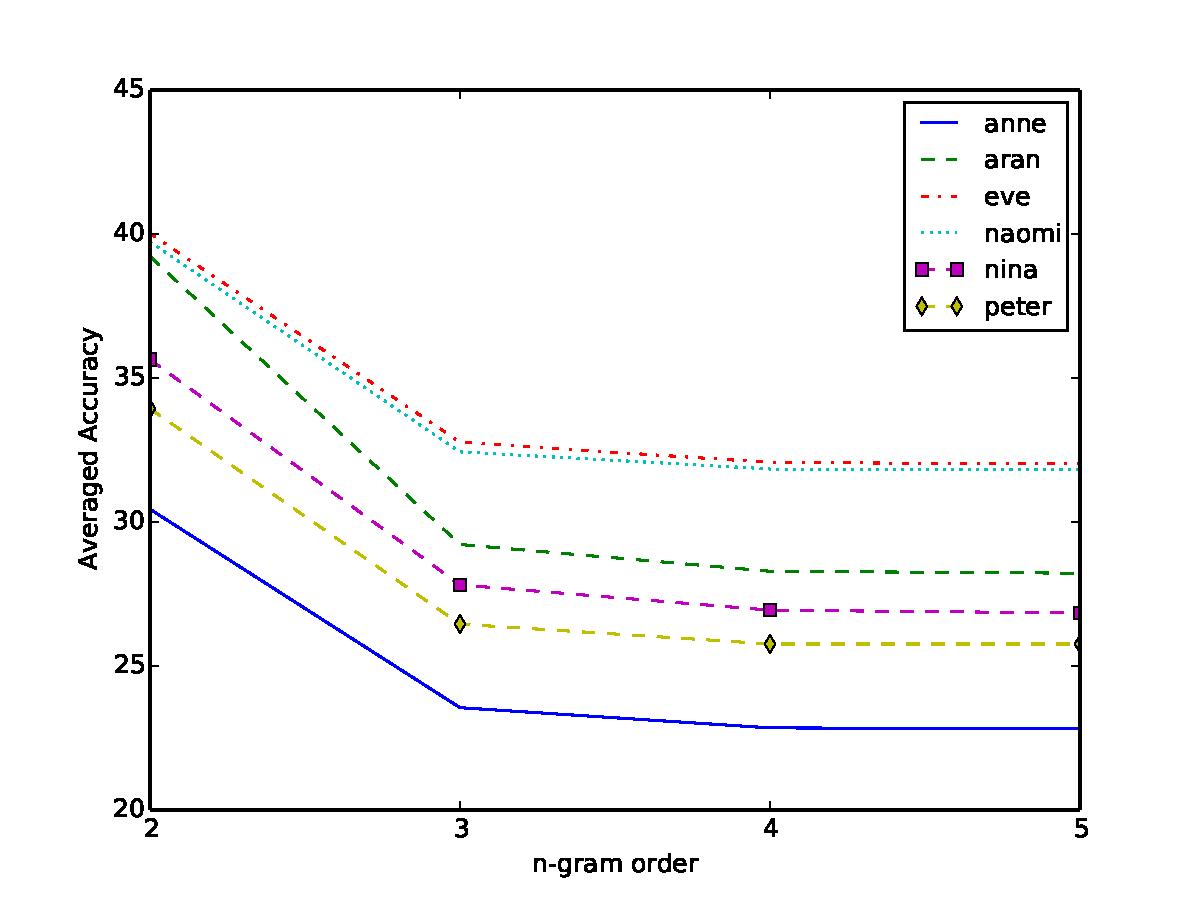
\includegraphics[width=.5\textwidth]{../figures/perplexity.pdf}
  \label{fig:perplexity}
  }
  \subfigure[]{
  \includegraphics[width=.5\textwidth]{../figures/ngram.pdf}
  \label{fig:ngram}
  }
  \caption{Language Model perplexities on each child corpus for different
  n-gram orders are presented on the left figure while 10-fold cross validation
  accuracies calculated based on these models are presented on the right.} 
\end{figure}

The perplexity of each child corpus is dramatically improved when the n-gram
order of the language model is increased from 2 to 3 and varies slightly for
orders higher than 3.  Figure~\ref{fig:perplexity} plots the perplexity versus
the n-gram order.  As shown in Figure~\ref{fig:ngram}, the model classification
accuracies on each child corpus are slightly improved for orders higher than 3
which is in fact parallel to the perplexity trends in
Figure~\ref{fig:perplexity}.  Overall, the classification accuracy of
paradigmatic model is highly correlated with the perplexity of the language
model that is used to sample substitutes.

%% One possible explanation of similar performances with n-grams 3,4 and 5 is
%% that our model defines the context of a target word by using $2n-2$ words
%% (i.e., $n-1$ words left to the target word and $n-1$ word right to the target
%% word) however most of the sentences in our test corpora is shorter than 7
%% words. 
%%% Presenting them with figure is much more powerful
%%% Perplexity of LM with different n-grams
%%\begin{table}[ht]
%%\centering
%%\caption{Language model perplexities on each child corpus for different n-gram
%%orders.} 
%%\begin{tabular}{lcccc}
%%  \hline  
%%  Child & 2-gram & 3-gram & 4-gram & 5-gram \\
%%  \hline
%%  Anne  & 30.44 & 23.55 & 22.85 & 22.81\\
%%  Aran  & 39.22 & 29.21 & 28.28 & 28.21\\
%%  Eve   & 40.02 & 32.77 & 32.06 & 32.01\\
%%  Naomi & 39.72 & 32.43 & 31.83 & 31.81\\
%%  Nina  & 25.64 & 27.81 & 26.93 & 26.84\\
%%  Peter & 33.93 & 26.45 & 25.76 & 25.76\\
%%  \hline
%%\end{tabular}
%%\label{t:perplexity}
%%\end{table}
%%
%%\begin{figure}[h]
%%  \subfigure[$aX$ model with $5K$ iterations] {
%%    \includegraphics[width=0.4\textwidth]{../figures/prtags5K.pdf}
%%    \label{fig:subfig5}
%%  }
%%  \subfigure[$Xb$ model with $5K$ iterations] {
%%    \includegraphics[width=0.4\textwidth]{../figures/pstags5K.pdf}
%%    \label{fig:subfig6}
%%  }
%%  \subfigure[$aXb$ model with $5K$ iterations] {
%%    \includegraphics[width=0.4\textwidth]{../figures/fretags5K.pdf}
%%    \label{fig:subfig7}
%%  }
%%  \subfigure[$aX+Xb$ model with $5K$ iterations] {
%%    \includegraphics[width=0.4\textwidth]{../figures/fletags5K.pdf}
%%    \label{fig:subfig8}
%%  }
%%  \subfigure[$a*b$ model with $5K$ iterations] {
%%    \includegraphics[width=0.4\textwidth]{../figures/wsubtags100K.pdf}
%%    \label{fig:subfig9}
%%  }
%%  \caption{10-fold cross validation individual tag accuracies of $aX$, $Xb$,
%%  $aXb$, $aX+Xb$ and $a*b$ on each child corpus after $5K$ iterations
%%  of feed-forward connectionist algorithm.}
%%  \label{fig:learningIteration5KApp}
%%\end{figure}
%%
%%\begin{figure}[h]
%%  \subfigure[$aX$ model with $100K$ iterations] {
%%    \includegraphics[width=0.4\textwidth]{../figures/prtags100K.pdf}
%%    \label{fig:subfig10}
%%  }
%%  \subfigure[$Xb$ model with $100K$ iterations] {
%%    \includegraphics[width=0.4\textwidth]{../figures/pstags100K.pdf}
%%    \label{fig:subfig11}
%%  }
%%  \subfigure[$aXb$ model with $100K$ iterations] {
%%    \includegraphics[width=0.4\textwidth]{../figures/fretags100K.pdf}
%%    \label{fig:subfig12}
%%  }
%%  \subfigure[$aX+Xb$ model with $100K$ iterations] {
%%    \includegraphics[width=0.4\textwidth]{../figures/fletags100K.pdf}
%%    \label{fig:subfig13}
%%  }
%%  \subfigure[$a*b$ model with $100K$ iterations] {
%%    \includegraphics[width=0.4\textwidth]{../figures/wsubtags100K.pdf}
%%    \label{fig:subfig14}
%%  }
%%  \caption{10-fold cross validation individual tag accuracies of $aX$, $Xb$,
%%  $aXb$, $aX+Xb$ and $a*b$ on each child corpus after $100K$ iterations
%%  of feed-forward connectionist algorithm.}
%%  \label{fig:learningIteration100KApp}
%%\end{figure}
% What happens when we change the data size?\\
% What happens when we change the vocabulary threshold?\\
% 
% \subsection{Input Corpora}
% \subsection{Method}
% \subsection{Results}
% 
% %% Let's drop this experiment, it is expensive.  We might handle 
% %% it hacking the fastsubs but I'm not sure about the mathematics.
% %% \section{Experiment 5}
% %% Left/rigth context substitute
% %% \subsection{Input Corpora}
% %% \subsection{Method}
% %% \subsection{Results}
% \section{Experiment 6}
% Other languages that we have in CHILDES
% 
% \section{Experiment 7}
% What happens if some of the words are given (semi-supervised setting)
% 
% \subsection{Input Corpora}
% \subsection{Method}
% \subsection{Results}



